\documentclass[12pt]{letter}\usepackage[letterpaper,margin=0.65in]{geometry}\usepackage{textcomp}\usepackage{graphicx}\usepackage[rflt]{floatflt}\pagenumbering{gobble}\begin{document}\begin{floatingfigure}{0.15\textwidth}\raisebox{0pt}[0pt][0pt]{\raisebox{-2.5cm}{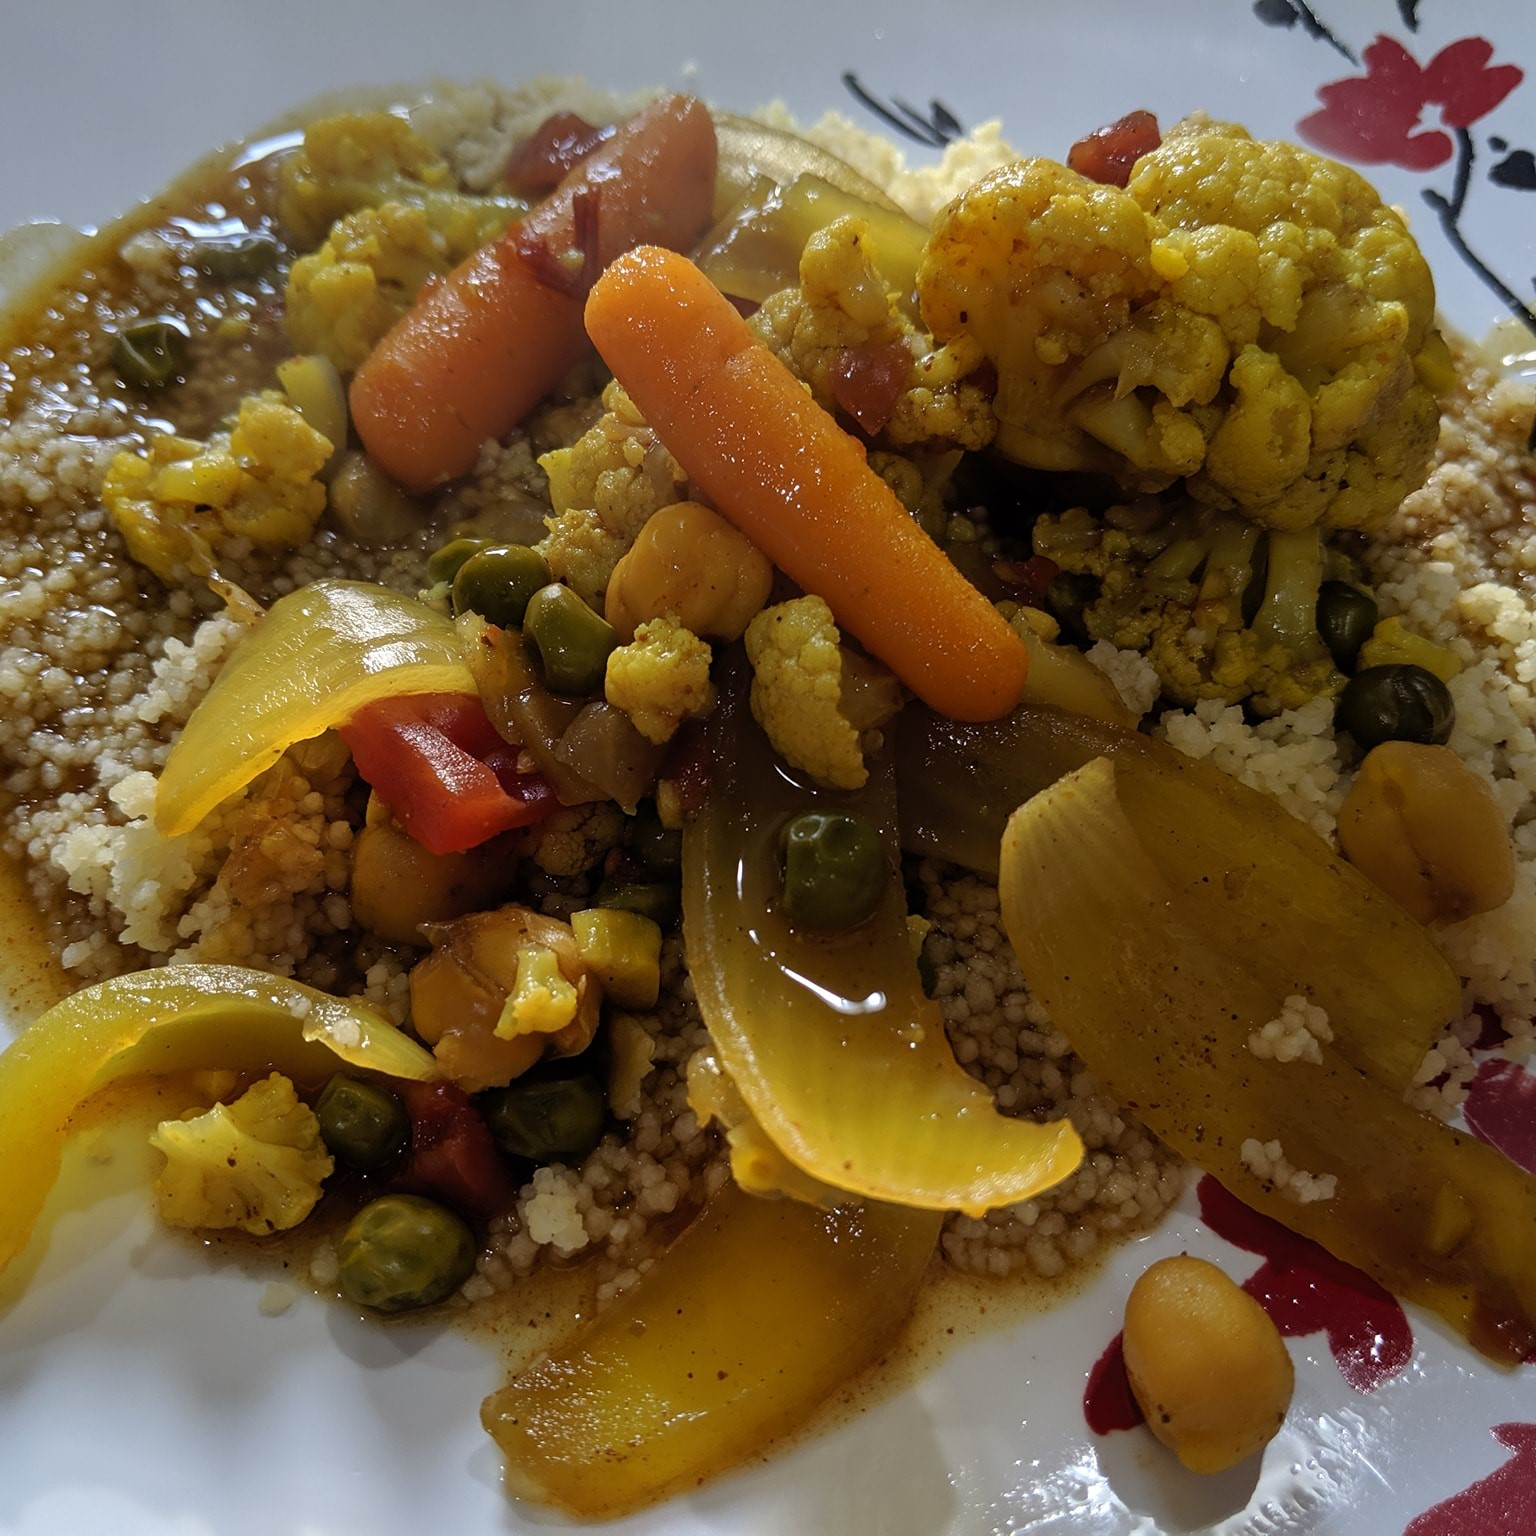
\includegraphics[width=0.15\textwidth]{moroccan-veggies}}}\end{floatingfigure}\begin{huge}Moroccan Veggies\end{huge}\newline\vspace{-2.5mm}\newline\renewcommand{\arraystretch}{1.1}\begin{tabular*}{\textwidth}{@{\extracolsep{\fill}}lr}A richly-flavored meal that's easy to prepare\\Sunny C\end{tabular*}\newline\vspace{10mm}\newline\begin{huge}Ingredients\end{huge}\\\rule[2.8mm]{\textwidth}{.1pt}\vspace{-3mm}\begin{itemize}\item 1 box vegetable broth\item 1 large head cauliflower, cut into florets\item 1 large yellow onion, coarsely chopped\item 25 baby carrots\item 1 can chickpeas, drained and rinsed\item 1 can diced tomatoes, drained\item 1 cup frozen peas\item 6 garlic cloves, minced\item 1 vegetable bouillon cube\item 1 teas turmeric\item $\frac{1}{2}$ teas ground cloves\item $\frac{1}{2}$ teas cinnamon\item $\frac{1}{2}$ teas chili powder\item $\frac{1}{4}$ teas ground ginger\end{itemize}\vspace{7mm}\begin{huge}Directions\end{huge}\\\rule[2.8mm]{\textwidth}{.1pt}\vspace{-3mm}\begin{enumerate}\item Pour vegetable broth into a large pan and whisk in seasonings.\item Add remaining ingredients and bring to a gentle boil.\item Reduce heat to low, and simmer (covered) until veggies are tender. Serve over couscous.\end{enumerate}\end{document}